\section{Electromyography} \label{sec:BG:EMG}

This project will utilize the method of electromyography to record the muscle activation of the lower arm muscles in relation to the movements presented in \secref{sec:BG:anatomy}. To develop theoretical background knowledge, a short introduction of the essentials of the signal will be presented. 

Electromyography is the recording of muscle activation. The amount of activity is found by measuring the electric potential, an action potential triggering a muscle contraction. The process of planning and executing a voluntary movement starts at the motor cortex in the brain, where a nerve impulse is send and travels through the spinal cord to the lower motor neuron. As seen in \figref{fig:motor} the path from alpha motor neuron through the axon to the motor endplates is what makes up a motor unit. The alpha motor neuron originates from the spinal cord along the axon to the muscle it controls. The axon branches out to multiple muscle fibers through motor endplates innervating the muscle fibers.
%Muscle movement demanding high precision have a higher innervation of motor units than muscles used for more powerful movements. 

\begin{figure}[H]                                         
	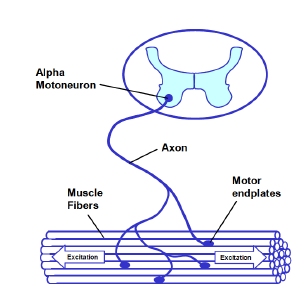
\includegraphics[width=.4\textwidth]{figures/motor_unit}  
	\caption{The figure illustrates the neural pathway from the alpha motor neuron to the innervated muscle fibers, making up a motor unit. \cite{Konrad2005}}
	\label{fig:motor} 
\end{figure}  

%The essentials of understanding the application EMG is the excitation of muscle cells. The excitability of the muscle fibers play a crucial role in a muscle contraction. The mechanisms of a contraction can be understood through a series of events. First the muscle cell membrane is at a resting potential between -80 to -90 mV, due to an equilibrium of NA$^+$ and K$^+$ through the intracellular and extracellular side of the membrane, maintained by an ion pump. The before mentioned alpha motor neuron reaches the motor endplates where a transmitter substance is released. The substance alters the membrane characteristics and allows a greater flow of Na$^+$ into the cell. This causes a membrane depolarization, changing the membrane potential. If a threshold between -55 mV to -50 mV is reached excitation in the form of an action potential is formed, travelling in both directions of the muscle fiber, as seen on \figref{fig:motor}. The membrane potential is quickly restored with a great outflow of Na$^+$, resulting in a repolarization. 

A fundamental part in the application of EMG is the understanding of the excitation of muscles. Muscles contract through a series of steps of changing potentials across muscle cell membranes and rapid polarization and repolarization. However, when recording EMG it is the superposition of the spread of the motor unit action potentials (MUAPs) over the muscle membrane that is recorded. \cite{Cram2012} 
Muscles are innervated by a varying number of nerves depending on the individual muscle. The MUAP is conducted to the muscle by nerves from the spinal cord, with the nerve impulses originating from the motor cortex in the brain. Muscles are not activated randomly by individual nerve fibers, but by nerves sorted into motor units. Many motor units are attached to a muscle and consist of a number of the nerves innervating the muscle. An illustration of how one motor unit attach to the muscle fibers of a muscle is illustrated in \figref{fig:motor}. When a motor unit activate, all the nerves in the motor unit is activated. This enables a controlled activation of the muscle as well as a activation that reach a higher number of muscle fibers. Motor units are also activated in an asynchronous pattern which enables different muscle fibers to be active at different times, making muscles less prone to fatigue. %The action potential from each of the activated muscle fibers summates spatially and temporally forming a motor unit action potential (MUAP). The spread of the MUAP over the muscle membrane is recorded with EMG.Regulating the number of recruited motor units is a way of controlling the force of a muscle contraction depended on the force needed. The frequency of motor unit activation can also be modulated for generating a specific amount of force. However, as different muscles recruit and activate muscle fibers at different frequencies, the amplitude and frequency visible from an EMG recording is necessary correlated with the generated muscle force. 
The force of a muscle contraction can be modulated either by motor unit recruitment or be frequency of activation. In EMG it is the sum of activity of activate motor units that is recorded. \cite{Cram2012}

In the scenario of this project multiple EMG electrodes will record signals from many muscles in the lower forearm. This will result in some muscles being active during some movements as they contract, while other muscles will be inactive. On an EMG recording this will be visible as contracting muscles will show high activity, while others will show little to no activity. An illustration of this can be seen on \figref{fig:EMGactivityExtensionFlexion}. The figure shows the muscle activity of muscles in the forearm when performing first extension at the wrist followed by flexion. As can be seen the muscle activity is very different between the two muscles. This enables the recognition of specific movements based on several EMG recordings with several different electrode placements. 
%The number of motor units innervating muscle fibers depend on the muscle characteristics and the purpose is serves. A low innervation ratio between motor units and muscle fibers gives the opportunity of fine motor tasks, while a low ratio is ideal for tasks demanding strength. Furthermore the motor units are recruited in an asynchronous pattern. This further facilitates the possibility of smooth muscle movements. \cite{Martini2012, Cram2012}

\begin{figure}[H] 
	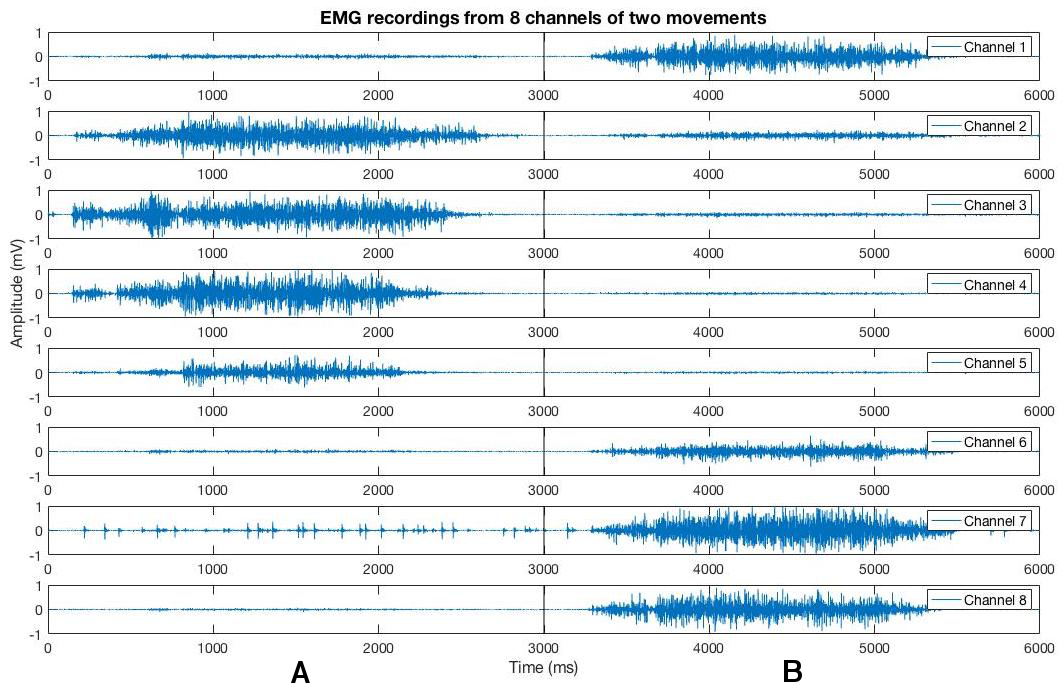
\includegraphics[width=0.9\textwidth]{figures/xBackground/EMGactivityExtensionFlexion}
	\caption{Illustration of the activity in an EMG recording of two movements: extension and flexion. Left side A) shows the activity recorded by EMG electrode channels during extension of the hand. Right side B) shows activity during flexion of the hand.}
	\label{fig:EMGactivityExtensionFlexion}
\end{figure}


Recording EMG can be done either through the most often used surface EMG (sEMG) or by intramuscular EMG (iEMG). In iEMG a needle is inserted into the muscle measuring the MUAP directly on site. The more often used sEMG that uses electrodes to measure the sum of MUAPs on the skin surface, will be used to acquire EMG signals in this project. \cite{Cram2012}
